\documentclass[12pt]{article}
\usepackage[utf8]{inputenc}
\usepackage[dutch]{babel}
\usepackage{algorithm}
\usepackage{algorithmic}
\usepackage{amssymb}
\usepackage{amsmath}
\usepackage{graphicx}

\author{Wolfgang M\"ollmann \& Robbe Degr\`eve}
\title{Toepassingen van meetkunde in de informatica \\ Project: Bepaling van het Dichtste Puntenpaar}

\begin{document}

\maketitle

\newpage

\section{Beschrijving van opstelling van puntenverzameling}
Voor het opstellen van een input-file met een aantal gegeven parameters om willekeurge punten te creëren gebruiken we de functie "makeRandom".
Deze functie zal de volgende parameters als input vragen:
\begin{enumerate}
    \item inFile: De puntenverzameling zal in dit bestand weggeschreven worden, indien het bestand niet bestaat zal het aangemaakt worden.
    \item alg: het nummer van het algoritme dat gebruikt moet worden: 1 (eenvoudige algoritme), 2 (eerste variante van het doorlooplijnalgoritme) of 3 (tweede variante van het doorlooplijnalgoritme)
    \item dim: de dimensie van de punten $M \geq 2$
		\item size: het aantal punten N
\end{enumerate}

Deze functie heeft als taak om een inputbestand op te stellen met willekeurge co\"ordinaten.
De functie zal de gegeven parameters eerst neerschrijven in de inFile.
Daarna gebeurd een initialisatie van \texttt{Random r}.
Daarna zullen we per regel van het bestand itereren van 0 tot en met de dimensie en voor iedere dimensie een willekeurige waarde neerschrijven in het bestand.
De willeukeurige co\"ordinaten kunnen waardes aannemen tussen $[0, 5[$.


\begin{algorithm}
\caption{De javafunctie \texttt{makeRandom}}
\begin{algorithmic}
\STATE \textbf{Input:} $inFile$, $alg$, $dim$, $size$
\STATE infile.println(alg)
\IF {$dim < 2$}
	\PRINT Dimension needs to be greater or equal to 2.
	\STATE \texttt{Exit}
\ENDIF
\STATE Random r = new Random()
\STATE $Iterator<Double> i$ = r.doubles(size * dim, 0.0, 5.0).iterator()
\STATE $String outString = ""$
\WHILE {$i.hasNext()$}
	\STATE $outString = ""$
	\FOR {$j = 0$; $j < dim$; j++}
		\STATE outString += String.format(Locale.US, "\%17.16f ", i.next())
	\ENDFOR
	\STATE inFile.println($outString$)
\ENDWHILE
\STATE inFile.flush()
\STATE inFile.close()
\end{algorithmic}
\end{algorithm}

\section{Opdracht 1: Hoog-niveau beschrijving van verscheidene algoritmes}

\subsection{Brute-force algorithm}

\subsubsection{hoogniveau beschrijving}

\begin{algorithm}
\caption{Bereken het dichtste puntenpaar met brute-force}
\begin{algorithmic}
	\STATE \textbf{Input:}  $rij$: Array met $N$ punten (gesorteerd naar stijgende x-co\"ordinaat)
  \STATE $d$ = $+\infty$
	\STATE $dpp1$ = 0, $dpp2$ = 0
  \STATE $currentDist$ = 0
  \FOR {$i$ to $length(rij)-1$}
    \FOR {$j = i + 1$ to $length(rij)$}
      \STATE $currentDist$ = calculate\_dist($rij[i]$, $rij[j]$)
      \IF {$currentDist < d$}
				\STATE $dpp1$ = $rij[i]$
				\STATE $dpp2$ = $rij[j]$
        \STATE $d$ = $currentDist$
  		\ENDIF
    \ENDFOR
  \ENDFOR
  \RETURN $dpp1$, $dpp2$, $d$
\end{algorithmic}
\end{algorithm}

\newpage
\subsection{Variant 1 algoritme}
\subsubsection{hoogniveau beschrijving}

\begin{algorithm}
\caption{Bereken het dichtste Puntenpaar volgens variant 1}
\begin{algorithmic}
	\STATE \textbf{Input:}  $rij$: Array met $N$ punten (gesorteerd naar stijgende x-co\"ordinaat)
	\STATE $d$ = $+\infty$
	\STATE $dpp1$ = 0, $dpp2$ = 0
	\STATE $currentDist$ = 0
	\FOR {$i = 1$ to $length(rij)$}
		\FOR {$j = i - 1$ to $0$}
		\IF {$rij[i].x - rij[j].x > d$}
			\STATE $break$
		\ENDIF
		\STATE $currentDist$ = calculate\_dist($rij[i]$, $rij[j]$)
			\IF {$currentDist < d$}
				\STATE $dpp1$ = $rij[i]$
				\STATE $dpp2$ = $rij[j]$
				\STATE $d$ = $currentDist$
			\ENDIF
		\ENDFOR
	\ENDFOR
	\RETURN $dpp1$, $dpp2$, $d$
\end{algorithmic}
\end{algorithm}

\subsubsection{rekencomplexiteit}

We zullen dus nagaan dat de rekencomplexiteit van dit algoritme gelijk is aan $O(N*Kgem)$.
We kunnen in het hoogniveau algoritme zien dat de eerste for-lus zal itereren over $N-1$ punten.
Voor elk van die punten zullen we dus de afstand bepalen van de punten die binnen de verticale strook V.
Indien we het $K_{gem}$ bepalen (uitgemiddeld over $i = 1,...,N$) zullen we een goede schatting hebben hoeveel punten er worden vergeleken in iedere iteratie van de doorlooplijn.
We rekenen bij $K_{gem}$ ook het eerste element bij die een $K$ zal hebben van 0, dus kunnen we bij onze doorloplijn iteratie het eerste punt ook meetellen.
We kunnen dus concluderen dat de rekencomplexiteit van variant 1 gelijk zal zijn aan $O(N*Kgem)$.

\subsection{worst-case puntenverzameling}

Voor de \textit{worst-case} puntenverzameling voor de eerste variant van het doorlooplijnalgoritme voor $M = 2$ hebben we een javafunctie \texttt{makeWorstCase}.
In deze functie maken een puntenverzameling aan van één kolom, waarbij alle punten dezelfde x-waarde hebben.
De y-waarde speelt hierbij geen rol.
In onze rij-implementatie sorteren we de punten met dezelfde x-waarden volgens de y-waarde.
Het tweede punt zal dus enkel vergelijken met het punt boven hem.
Het derde punt zal nadien vergelijken met het eerste en het tweede punt.
Uiteindelijk zal het laatste (onderste) punt zal dus met alle punten vergelijken.
Dit zal ons uiteindelijk $\frac{(n+1)}{2}$ vergelijkingen geven. De rekencomplexiteit zal dus $O(n^2)$ zijn.
Voor Kavg kunnen we concluderen dat per N het aantal kavg voor de worst-case gelijk zal zijn aan $\frac{N-1}{2}$.
Kavg zal dus voor de worst-case in 2 dimesies een stijgend karakter hebben, wat in tegenstelling is tot willekeurige puntenverzamelingen in 2 dimensies (zie figuur 3).
Dat is ook logisch. We hebben daarnet geconcludeerd dat de rekentijd van variant 1 van de worst-case zal toenemen in verband met het aantal punten.
De rekencomplexiteit is gelijk aan $(N*K_{avg})$, hieruit kunnen we zien dat voor een stijgende rekencomplexiteit we ook een stijgende Kavg nodig zullen hebben.
Kmax zal ook een stijgend karakter hebben. We kunne afleiden dat voor iedere N de Kmax steeds gelijk zal zijn aan $N-1$.
Voor de worst-case zal het laatste punt dat gecontroleerd moet worden de afstand berekenen met alle vorige punten.


\subsection{Variant 2 algorithm}
\subsubsection{hoogniveau beschrijving}

\begin{algorithm}
\caption{Bereken het dichtste Puntenpaar volgens variant 2}
\begin{algorithmic}
	\STATE \textbf{Input:}  $rij$: Array met $N$ punten (gesorteerd naar stijgende x-co\"ordinaat)
	\STATE $d$ = $+\infty$
	\STATE $dpp1$ = 0, $dpp2$ = 0
	\STATE $currentDist$ = 0
	\STATE $t$: gegevensstructuur waarin punten links van de doorlooplijn opgeslagen zijn, gesorteerd naar stijgende y-coordinaat
  \FOR {$i = 1$ to $length(rij)-1$}
    \STATE voegtoe($t, rij[i-1]$)
    \STATE $low = rij[i]$
    \STATE $low.y = low.y - d$
    \STATE $next = boven(t,low)$
    \WHILE {$next \neq Null \textrm{ AND } next.y < rij[i].y + d$}
      \IF {$next.x < rij[i].x - d$}
        \STATE verwijder($t, next$)
        \STATE $next = boven(t,next)$
        \STATE $continue$
      \ENDIF
      \STATE $currentDist$ = calculate\_dist($rij[i]$, $next$)
  	  \IF {$currentDist < d$}
  			\STATE $dpp1$ = $rij[i]$
  			\STATE $dpp2$ = $next$
  			\STATE $d$ = $currentDist$
  		\ENDIF
      \STATE $next = boven(t,next)$
    \ENDWHILE
  \ENDFOR
\end{algorithmic}
\end{algorithm}

\subsection{rekencomplexiteit}
De behandeling van ieder punt p zal gemiddeld O(logN) bewerkingen nodig hebben.
We maken bij onze variant 2 gebruik van een gebalanceerde zoekboom.
We weten dat alle nodige bewerkingen in O(logK) operaties kunnen uitgevoerd worden in de boom.
Het algoritme voegt bij elke iteratie het punt dat we aan het behandelen zijn toe aan de boom.
Bij de behandeling van het laatste punt zullen we alle punten toegevoegd hebben aan de boom.
Voor het laatste punt zal dus elke bewerking log(N) tijd kosten.



\section{Grafieken}

\subsection{veronderstelling}
Indien we spreken over rekencomplexiteit bedoelen we de complexiteit van het algoritme zonder de rekentijd van het sorteren van de input.
Bij tijdscomplexiteit maken we de som tussen rekentijd van het sorteren en de rekentijd van het algoritme zelf.

\subsection{figuur 1}
In Figuur 1 zullen we de rekentijden tussen het brute-force algoritme en variant1 vergelijken.
We zullen op de x-as het aantal punten uitzetten.
De gekozen aantal punten zijn logaritmisch bepaald met als basis 1.1 beginnend vanaf 302 tot en met 12279.
Op de y-as zetten we de rekentijd uit in milliseconden. Hiervoor gebruiken we een logaritmische functie met basis 2.
We kunnen concluderen uit deze plot dat variant 1 voor alle onze gekozen punten een effeciënter algoritme is.
We kunnen ook zien dat de het brute-force algoritme een steiler verloop heeft, hieruit kunnen we afleiden dat voor zeer grote aantallen punten het verschil tussen de twee algoritmes steeds groter zal worden.

\begin{figure}
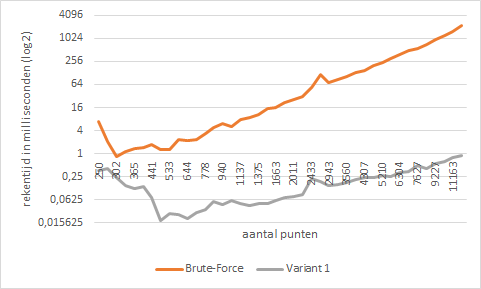
\includegraphics[width=\textwidth]{Simpel-var1-rekentijd.png}
\caption{De plot van de rekentijden tussen het brute-force algoritme en variant 1 voor 2 dimensies}
\end{figure}

\subsection{figuur 2}

In figuur 2 zullen we het verband tussen de Kmax en het aantal punten plotten.
Op de x-as zetten we het aantal punten uit van 250 tot 12279 met een logaritmische functie met basis 1,1.
Op de y-as zetten we de Kmax uit die in dit geval zal gaan van een minimum van 2 tot en met een maximum van 25.
We kunnen op de plot zien dat de grafiek Kmax een licht stijgend karakter heeft.
We kunnen wel zien dat steeds Kmax relatief klein zal blijven ten opzichte van het aantal punten.

\begin{figure}
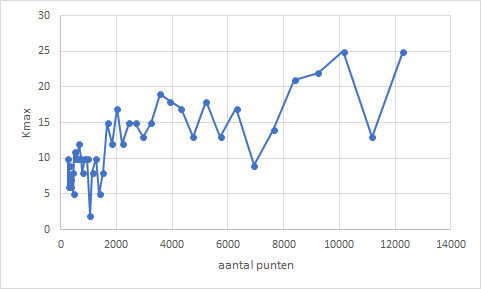
\includegraphics[width=\textwidth]{punten-Kmax.png}
\caption{De plot tussen het aantal punten en Kmax voor 2 dimensies}
\end{figure}

\subsection{figuur 3,4 en 5}

In figuur 3 zullen we het verband tussen de Kavg en het aantal punten plotten.
Op de x-as zetten we het aantal punten uit van 250 tot 12279 met een logaritmische functie met basis 1.1.
Op de y-as zetten we de Kmax uit die in dit geval zal gaan van een minimum van 0,1480 tot en met een maximum van 2,14186.
Op deze plot is duidelijk te herkennen dat Kavg ongeveer constant zal blijven ongeacht het aantal punten.
In ons experiment was deze constante 1,35.
We kunnen concluderen dat voor willekeurige puntenverzameling in 2 dimensies de Kavg zeer klein zal zijn in vergelijkign met N.

In Figuur 4 zullen we de het aantal dimensies plotten in functie van de rekentijd voor variant 1.
We zullen op de x-as het aantal dimensies uitzetten van 2 tot en met 19.
Op de y-as zetten we de rekentijd uit in milliseconden.
We zien duidelijk dat voor een stijgende M gaat het voordeel van het doorlooplijn verloren.
Dit kunnen we eenvoudig bepalen aan de hand van de rekencomplexiteit en figuur 5.

In figuur 5 zien we dat Kavg een lineair verband heeft met het aantal dimensies.
We weten ook dat de rekencomplexiteit van variant 1 gelijk is aan O(N*Kavg).
Hierdoor kunnen we dus afleiden dat de rekencomplexiteit ook zal stijgen in functie het aantal dimensies.
\\TODO Waarom? Voor welke waarde van M is er geen voordeel meer? Waarom?

\begin{figure}
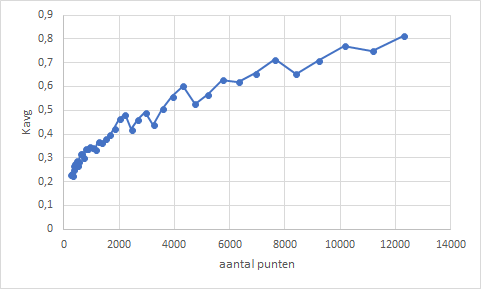
\includegraphics[width=\textwidth]{punten-Kavg}
\caption{De plot tussen het aantal punten en Kavg voor 2 dimensies}
\end{figure}

\begin{figure}
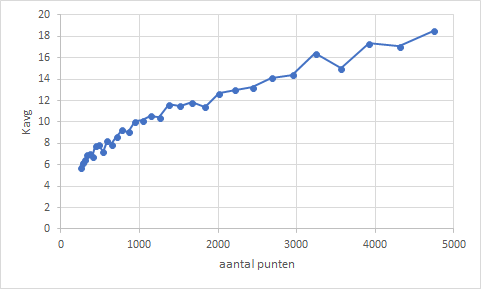
\includegraphics[width=\textwidth]{punten-Kavgdim3.png}
\caption{De plot tussen het aantal punten en Kavg voor 3 dimensies}
\end{figure}

\begin{figure}
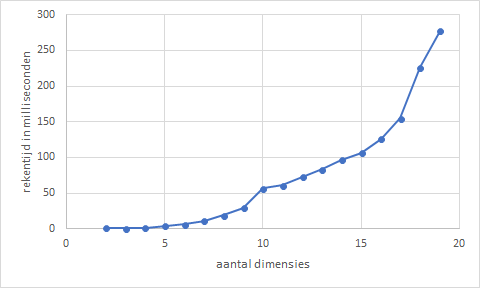
\includegraphics[width=\textwidth]{dim-var1-rekentijd.png}
\caption{De plot tussen het aantal dimensies en de rekentijd van variant 1 (voor 2500 punten)}
\end{figure}

\subsection{figuur 6}

In figuur 6 zullen we het verband tussen de Kavg en het aantal dimensies plotten.
Op de x-as zetten we het aantal dimensies uit van 2 tot 19.
Op de y-as zetten we de Kavg uit.
Op deze plot is duidelijk te herkennen dat Kavg ongeveer constant zal blijven ongeacht het aantal punten.
In ons experiment was deze constante 1,35.
We kunnen concluderen dat voor willekeurige puntenverzameling in 2 dimensies de Kavg zeer klein zal zijn in vergelijkign met N.




\begin{figure}
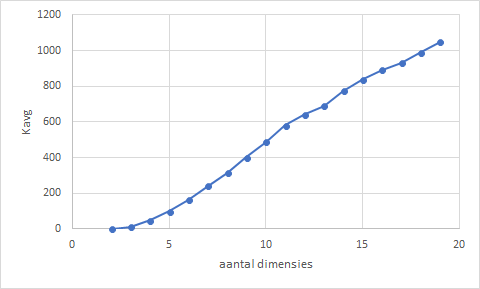
\includegraphics[width=\textwidth]{dim-Kavg.png}
\caption{De plot tussen het aantal dimensies en Kavg (voor 2500 punten)}
\end{figure}

\subsection{figuur 7}





\begin{figure}
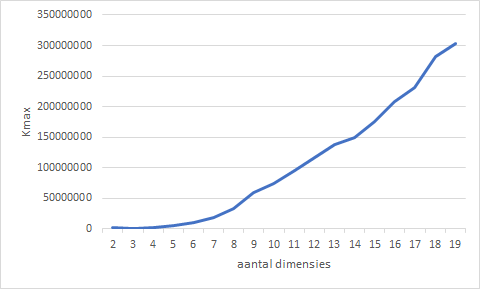
\includegraphics[width=\textwidth]{dim-Kmax.png}
\caption{De plot tussen het aantal dimensies en Kmax (voor 2500 punten)}
\end{figure}









\end{document}
